\section{Τεχνολογίες υλοποίησης} \label{subsection:4-2-implementation-technology-stack}

Η παρούσα ενότητα απαρτίζεται από υποενότητες, στις οποίες διατυπώνονται οι \textbf{σημαντικότερες} τεχνολογίες που χρησιμοποιήθηκαν για την υλοποίηση της εφαρμογής. Όλες οι τεχνολογίες αποτελούν δωρεάν λογισμικό ανοιχτού κώδικα.

\subsection{Τεχνολογίες σχετικές με το development}

Σε αυτήν την υποενότητα περιγράφονται ορισμένα θεμελιώδη εργαλεία και frameworks που συνετέλεσαν στην ανάπτυξη της εφαρμογής.

%TODO: Add janus and build steps diagram

\subsubsection{Node.js} \label{subsection:4-2-1-1-node.js}

\logo{chapter-4/4.2.node.js-logo}{Node.js logo}

Το Node.js\footnote{\url{https://nodejs.org/}} είναι ένα περιβάλλον χρόνου εκτέλεσης JavaScript πολλαπλών πλατφορμών, το οποίο εκτελείται στη μηχανή V8\footnote{\url{https://v8.dev/}} και παρέχει τη δυνατότητα εκτέλεσης κώδικα JavaScript εκτός περιηγητών ιστού. Επιτρέπει στους προγραμματιστές να χρησιμοποιούν JavaScript για τη σύνταξη εργαλείων γραμμής εντολών και τη δημιουργία κλιμακωτών διαδικτυακών εφαρμογών (κυρίως για εξυπηρετητές). Έχει αρχιτεκτονική βασισμένη σε συμβάντα (event-driven architecture), με δυνατότητα ασύγχρονης εισόδου/εξόδου (asynchronous I/O).\cite{4.2-node.js}

Ένα από τα σημαντικότερα χαρακτηριστικά του Node.js είναι ο ενσωματωμένος διαχειριστής πακέτων του, ο οποίος ονομάζεται npm. Με τον npm γίνεται εφικτή η εγκατάσταση πακέτων (βιβλιοθηκών) από το μητρώο npm (npm registry\footnote{\url{https://www.npmjs.com/}}), καθώς και η οργάνωση και η διαχείρισή τους στα πλαίσια της ανάπτυξης μίας εφαρμογής που εξαρτάται από αυτά.

Το Node.js έχει το αποθετήριό του στο GitHub\footnote{\url{https://github.com/nodejs/node}}.
\subsubsection{Docker} \label{subsection:4-2-1-2-docker}

\logo{chapter-4/4.2.docker-logo}{Docker logo}

Το Docker\footnote{\url{https://www.docker.com/}} αποτελεί μία πλατφόρμα η οποία παρέχει λογισμικό εικονοποίησης (virtualization) στο επίπεδο του λειτουργικού συστήματος καθώς και ολοκληρωμένα συστήματα διαμοιρασμού και εκτέλεσης των παραγόμενων εικόνων.

Δίνει την δυνατότητα σύνθεσης εικονικών περιβαλλόντων λειτουργικού συστήματος τα οποία ονομάζονται εικόνες (images). Μέσα στις εικόνες είναι δυνατή η εκτέλεση προγραμμάτων σε ασφαλή, απομονωμένα και προβλέψιμα περιβάλλοντα τα οποία εγγυούνται τις ίδιες συνθήκες εκτέλεσης παντού. Έτσι, οι προγραμματιστές δεν χρειάζεται να ανησυχούν για το περιβάλλον εκτέλεσης του κώδικα και την ρύθμιση των παραμέτρων σε κάθε ξεχωριστή εγκατάσταση.

Ταυτόχρονα, η πλατφόρμα του Docker παρέχει συστήματα και τυποποιημένες μεθόδους για το πακετάρισμα των εικόνων, την μεταφόρτωση και την εκτέλεσή τους σε απομακρυσμένα συστήματα. Με αυτό τον τρόπο αποτελεί πολύτιμο εργαλείο το οποίο έχει γίνει το στάνταρ στη βιομηχανία λογισμικού για τον διαμοιρασμό και την εγκατάσταση ολοκληρωμένων εφαρμογών σε περιβάλλοντα δοκιμής (staging environments) και παραγωγής (production environment).

Τέλος, η δυνατότητα τοπικής εκτέλεσης των εικόνων στο σύστημα ανάπτυξης του κώδικα δίνει την ευκαιρία ελέγχου (testing) και αποσφαλμάτωσης (debug) τοπικά σε ένα περιβάλλον ίδιο με αυτό της εκτέλεσης. Αυτό είναι εξαιρετικά σημαντικό επειδή αποκλείει τυχών μεταβολές στην πορεία εκτέλεσης του προγράμματος που μπορεί να έρχονταν από την εκτέλεση σε ένα διαφορετικό περιβάλλον.

% TODO: example citations
% Merkel, Dirk. “Docker: Lightweight Linux Containers for Consistent Development and Deployment.” Linux Journal, vol. 2014, no. 239, 2014, p. 2.
% Anderson, Charles. “Docker [Software Engineering].” IEEE Software, vol. 32, no. 3, 2015.

\subsubsection{Jenkins} \label{subsection:4-2-1-3-jenkins}

\logo{chapter-4/4.2.jenkins-logo}{Jenkins logo}

Το Jenkins είναι ένας πλήρως παραμετροποιήσιμος και επεκτάσιμος διακομιστής αυτοματοποίησης (automation server). Ο διακομιστής μπορεί να αυτοματοποιήσει τις διαδικασίες ελέγχου, ολοκλήρωσης, παράδοσης και εγκατάστασης του κώδικα, υλοποιώντας έτσι βασικές διαδικασίες που ορίζει το DevOps, συνεχή έλεγχο (continuous testing), συνεχή ολοκλήρωση (continuous integration), συνεχή παράδοση (continuous delivery) και συνεχή εγκατάσταση (continuous deployment). Επίσης, το Jenkins μπορεί να παραμετροποιηθεί μέσω των ρυθμίσεων που προσφέρει και των επεκτάσεων (plugins) που υπάρχουν ώστε να παρέχει τις δυνατότητες αυτές για οποιαδήποτε πλατφόρμα, γλώσσα και περιβάλλον ανάπτυξης.

Στο Jenkins είναι δυνατός ο ορισμός με χρήση κώδικα (σε Groovy και στο DSL που παρέχεται από το Jenkins) πολλαπλών γραμμών εργασιών (pipeline). Οι γραμμές εργασιών συντίθενται από πολλαπλά βήματα τα οποία επιτελούν ξεχωριστούς στόχους προς το τελικό αποτέλεσμα της γραμμής. Τα βήματα μπορούν να τρέχουν σειριακά ή παράλληλα. Ενώ δίνεται η δυνατότητα εκτέλεσης σε πολλαπλά, διανεμημένα συστήματα καθώς και άλλες προχωρημένες λειτουργικότητες.

Το Jenkins συνδυάζεται αποτελεσματικά με την πλατφόρμα του Docker που περιγράφηκε προηγουμένως. Μέσω του συνδυασμού δίνεται η ευκαιρία της αυτοματοποίησης του μεγαλύτερου μέρους του DevOps σε ένα απολύτως προβλέψιμο περιβάλλον το οποίο παραμένει σταθερό από την ανάπτυξη του κώδικα μέχρι την τελική εγκατάσταση. Με αυτή την μέθοδο βελτιώνεται σημαντικά η αποτελεσματικότητα των ομάδων ανάπτυξης κώδικα.

% example citations
% Shahin, Mojtaba, et al. “Continuous Integration, Delivery and Deployment: A Systematic Review on Approaches, Tools, Challenges and Practices.” IEEE Access, vol. 5, 2017, pp. 3909–3943.
% Meyer, Mathias. “Continuous Integration and Its Tools.” IEEE Software, vol. 31, no. 3, 2014, pp. 14–16.
% Virmani, Manish. “Understanding DevOps & Bridging the Gap from Continuous Integration to Continuous Delivery.” Fifth International Conference on the Innovative Computing Technology (INTECH 2015), 2015, pp. 78–82.


\subsection{Τεχνολογίες σχετικές με το UI}

Στην παρούσα υποενότητα περιγράφονται όσες τεχνολογίες σχετίζονται με τη διεπαφή του χρήστη (UI), δηλαδή με το Presentation tier.

% TODO: add technologies like redux, sagas

\subsubsection{React} \label{subsection:4-2-2-1-react}

\logo{chapter-4/4.2.react-logo}{React logo}

Η React\footnote{\url{https://reactjs.org/}} αποτελεί βιβλιοθήκη JavaScript, η οποία χρησιμοποιείται για την κατασκευή διεπαφών χρήστη. Είναι δηλωτική (declarative) και βασίζεται σε components, τα οποία διαχειρίζονται την κατάστασή τους (state) και συντίθενται για να δημιουργήσουν πολύπλοκα διαδραστικά UIs. Τα components συνήθως υλοποιούνται σε JSX (JavaScript Syntax Extension), η οποία επεκτείνει τη JavaScript, επιτρέποντας την εισαγωγή αυτούσιων HTML εκφράσεων εντός του κώδικά της.

Ένα σημαντικό εργαλείο για την ταχεία ανάπτυξη web εφαρμογών σε React είναι το Create React App\footnote{\url{https://create-react-app.dev/}}. Με τη χρήση μίας και μόνο εντολής (\texttt{npx create-react-app my-app}), εγκαθίσταται αυτόματα ένας development server σε περιβάλλον Node.js (ως μία μοναδική βιβλιοθήκη). Αυτός εμπεριέχει μία πληθώρα από build tools (π.χ. Webpack, Babel, ESLint), τα οποία προσφέρουν ισχυρές δυνατότητες, όπως άμεσα reloads και παραγωγή βελτιστοποιημένων bundles. Έτσι, η διαδικασία της υλοποίησης αποκτά ποικίλες διευκολύνσεις, χωρίς να απαιτεί την εκμάθηση, την χειροκίνητη εγκατάσταση και την προηγμένη διαμόρφωση των τεχνολογιών στο εσωτερικό. 

Η React έχει το αποθετήριό της στο GitHub (\url{https://github.com/facebook/react/}) και διατίθεται μέσω του μητρώου npm (\url{https://www.npmjs.com/package/react}).

\subsubsection{Redux} \label{subsection:4-2-2-2-redux}

\logo{chapter-4/4.2.redux-logo}{Redux logo}

Το Redux\footnote{\url{https://redux.js.org/}} αποτελεί μία βιβλιοθήκη JavaScript, η χρήση της οποίας προσφέρει στην εφαρμογή ένα πλήρως διαχειρίσιμο global state.

Τα δομικά στοιχεία του Redux είναι τα εξής:
\begin{itemize}
	\item \textbf{Actions}: Αντικείμενα τα οποία περιέχουν νέα πληροφορία για την τροποποίηση του state της εφαρμογής.
	\item \textbf{Reducers}: Συναρτήσεις, οι οποίες λαμβάνοντας ένα action και διαβάζοντας το τρέχον state, εφαρμόζουν κάποια λογική για την παραγωγή ενός νέου state.
	\item \textbf{Store}: Το αντικείμενο στο οποίο βρίσκεται αποθηκευμένο το state της εφαρμογής. Η βασική ιδιότητα του state είναι ότι παραμένει αμετάβλητο και, για την ανανέωσή του, παράγεται πάντα ένα νέο state object μέσω των reducer.
	\item \textbf{Middleware}: Προαιρετικά κομμάτια κώδικα που λαμβάνουν actions πριν εκείνα φτάσουν στους reducer και τα οποία εκτελούν κάποιο side effect. Συνήθως χρησιμοποιούνται για ενέργειες όπως logging και error reporting, ή για να ενώσουν το Redux με εξωτερικά API. 
\end{itemize}

Αν και το ίδιο το Redux είναι μικροσκοπικό σε μέγεθος, ο τρόπος υλοποίησής του έχει επιτρέψει τη δημιουργία ενός τεράστιου οικοσυστήματος εργαλείων και επεκτάσεων, τα οποία συνδέονται μαζί του ή βασίζονται σε αυτό. Για παράδειγμα, μία από τις κύριες χρήσεις του είναι η κατασκευή διεπαφών χρήστη σε συνδύασμό με άλλες βιβλιοθήκες, όπως με τη React. Σε αυτήν την περίπτωση, συνδέεται μαζί της με το npm πακέτο \texttt{react-redux} και η λειτουργία του υπό ανάπτυξη UI προκύπτει ως εξής:

\begin{figure}[H]
	\centering
	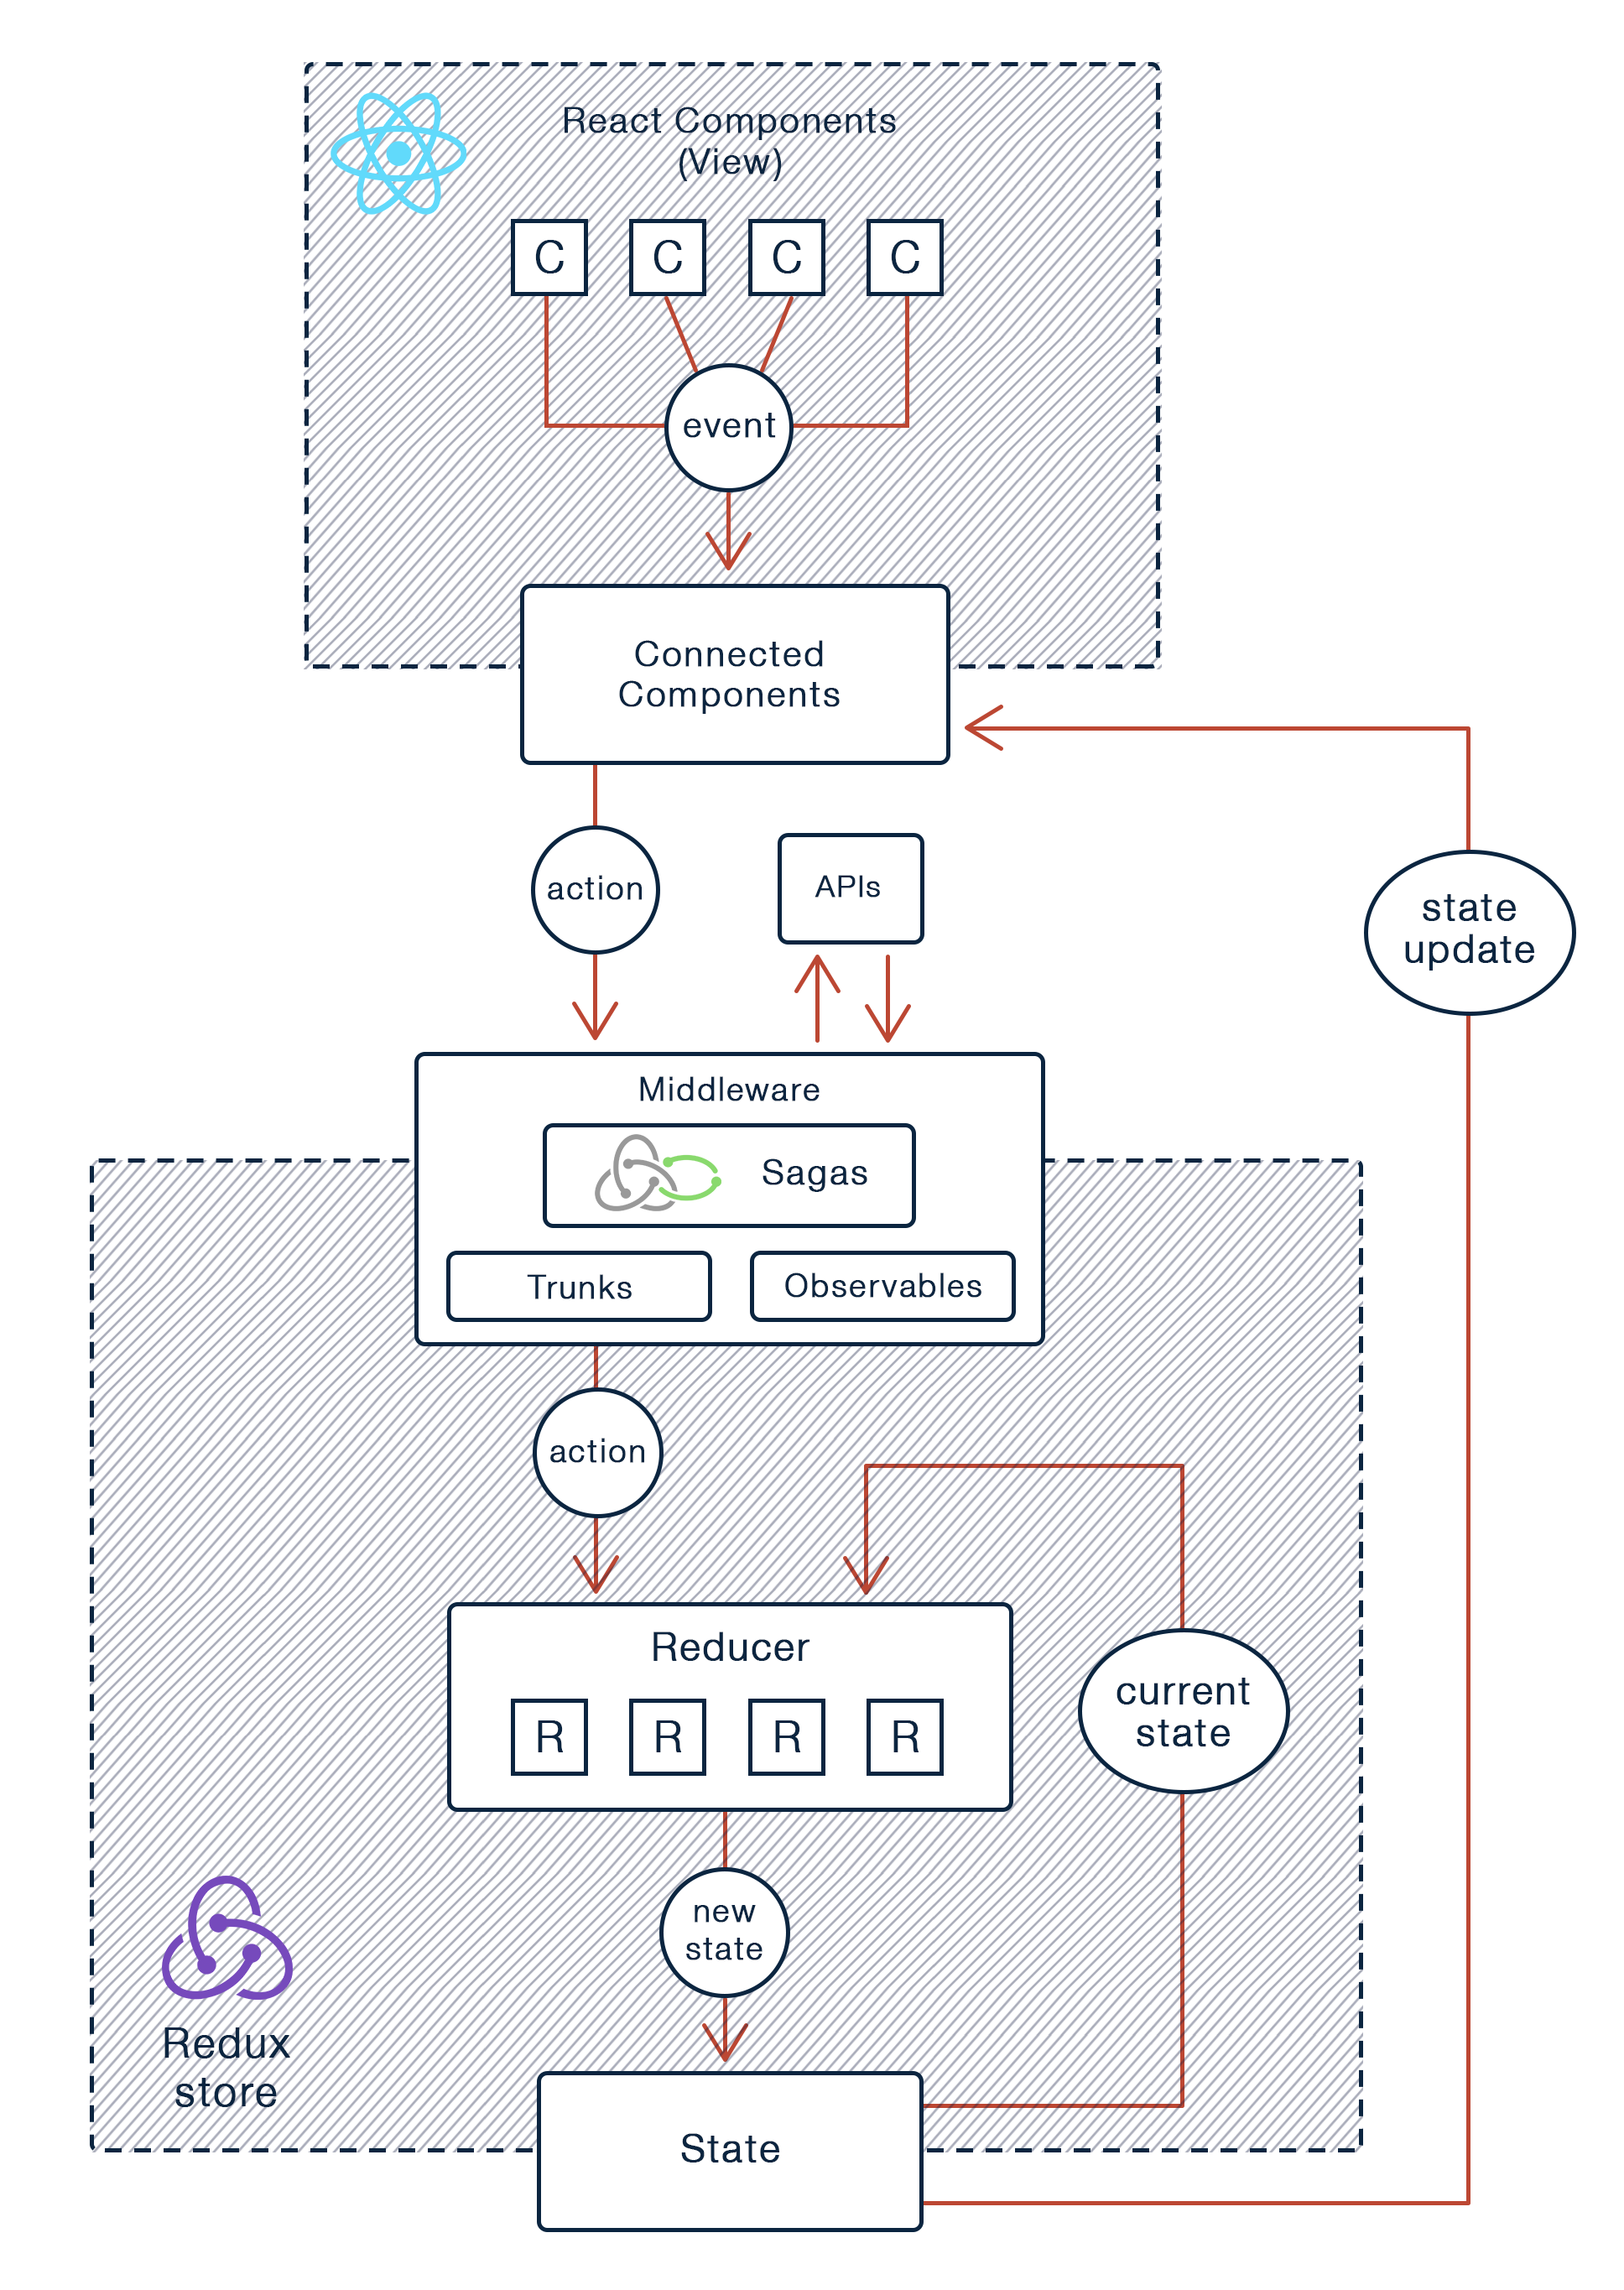
\includegraphics[width=.9\textwidth]{assets/figures/chapter-4/4.2.react-redux}
	\caption{Λειτουργία του Redux σε συνδυασμό με React}
\end{figure}
\vspace{\parskip}
Το Redux έχει το αποθετήριό του στο GitHub\footnote{\url{https://github.com/reduxjs/redux}} και διατίθεται μέσω του μητρώου npm\footnote{\url{https://www.npmjs.com/package/redux}}.

\subsubsection{Redux-Saga} \label{subsection:4-2-2-3-redux-saga}

\logo{chapter-4/4.2.redux-saga-logo}{Redux-Saga logo}

Το Redux-Saga\footnote{\url{https://redux.js.org/}} αποτελεί μία βιβλιοθήκη JavaScript του οικοσυστήματος του Redux. Πρόκειται για ένα Redux middleware, το οποίο χρησιμοποιεί ESG generator functions\footnote{\url{https://developer.mozilla.org/en-US/docs/Web/JavaScript/Reference/Statements/function*}} για την εκτέλεση και διαχείριση ποικίλων ασύγχρονων side effect. Αυτές οι συναρτήσεις (sagas) παρέχουν μία πληθώρα επιλογών για την παράλληλη εκτέλεση κώδικα που μπορεί να σχετίζεται με εξωτερικά APIs, όπως με ένα blockchain ή μία βάση δεδομένων. Με αυτόν τον τρόπο, τα τελευταία μπορούν να συμπεριληφθούν στο κεντρικό Redux store και τη διαχείριση του συνολικού state της εφαρμογής.

Το Redux-Saga έχει το αποθετήριό του στο GitHub\footnote{\url{https://github.com/redux-saga/redux-saga}} και διατίθεται μέσω του μητρώου npm\footnote{\url{https://www.npmjs.com/package/redux-saga}}.

\subsection{Τεχνολογίες σχετικές με το Ethereum} \label{subsection:4-2-3-ethereum-technologies}

Στην παρούσα υποενότητα περιγράφονται εκείνες οι τεχνολογίες που σχετίζονται με το Ethereum, δηλαδή με το Application tier της τεχνολογικής στοίβας.

\subsubsection{Truffle} \label{subsection:4-2-3-1-truffle}

\logo{chapter-4/4.2.truffle-logo}{Truffle logo}

Το Truffle\footnote{\url{https://trufflesuite.com/truffle/}} είναι ένα από τα δημοφιλέστερα Ethereum development framework και αποτελεί τμήμα της σουίτας Truffle.

Μέσω του Truffle πραγματοποιείται η διαχείριση των έξυπνων συμβολαίων. Αυτή περιλαμβάνει τόσο τη δοκιμή, τη σύνδεση και τη μεταγλώττισή τους, όσο και την εγκατάστασή τους στο blockchain.

Επίσης, το Truffle περιέχει πρόσθετα σχετικά εργαλεία, όπως διαδραστική κονσόλα για άμεση αλληλεπίδραση με τα contract και εκτελεστή εξωτερικών σεναρίων (external script runner). 

Έχει το αποθετήριό του στο GitHub\footnote{\url{https://github.com/trufflesuite/truffle}} και διατίθεται μέσω του μητρώου npm\footnote{\url{https://www.npmjs.com/package/truffle}}.
\subsubsection{Ganache} \label{subsection:4-2-3-2-ganache}

\logo{chapter-4/4.2.ganache-logo}{Ganache logo}

Το Ganache\footnote{\url{https://trufflesuite.com/ganache/}} είναι ένα λογισμικό που παρέχει ένα βοηθητικό προσωπικό Ethereum blockchain για ταχεία ανάπτυξη αποκεντρωμένων εφαρμογών και αποτελεί επίσης τμήμα της σουίτας Truffle. Διατίθεται τόσο ως desktop εφαρμογή με UI, όσο και ως CLI (command-line interface).

To Ganache παρέχει ισχυρά εργαλεία για την ανάπτυξη έξυπνων συμβολαίων, όπως:
\begin{itemize}
	\item Block explorer, μέσω του οποίου μπορούν να εξεταστούν λεπτομερώς όλα τα blocks και οι συναλλαγές που έλαβαν χώρα.
	\item Εξρεύνηση των εσωτερικών των contracts και των πυροδοτημένων event τους.
	\item Ενδελεχές αρχείο καταγραφής της εξόδου του blockchain, το οποίο περιλαμβάνει σημαντικές πληροφορίες για τον εντοπισμό σφαλμάτων.
	\item Δυνατότητα διαμόρφωσης του χρόνου εξόρυξης των block, έτσι ώστε να αρμόζει με τις εκάστοτε ανάγκες (αυτόματη εξόρυξη ή εξόρυξη σε προσαρμοσμένο χρονικό διάστημα).
\end{itemize}

\begin{figure}[H]
	\centering
	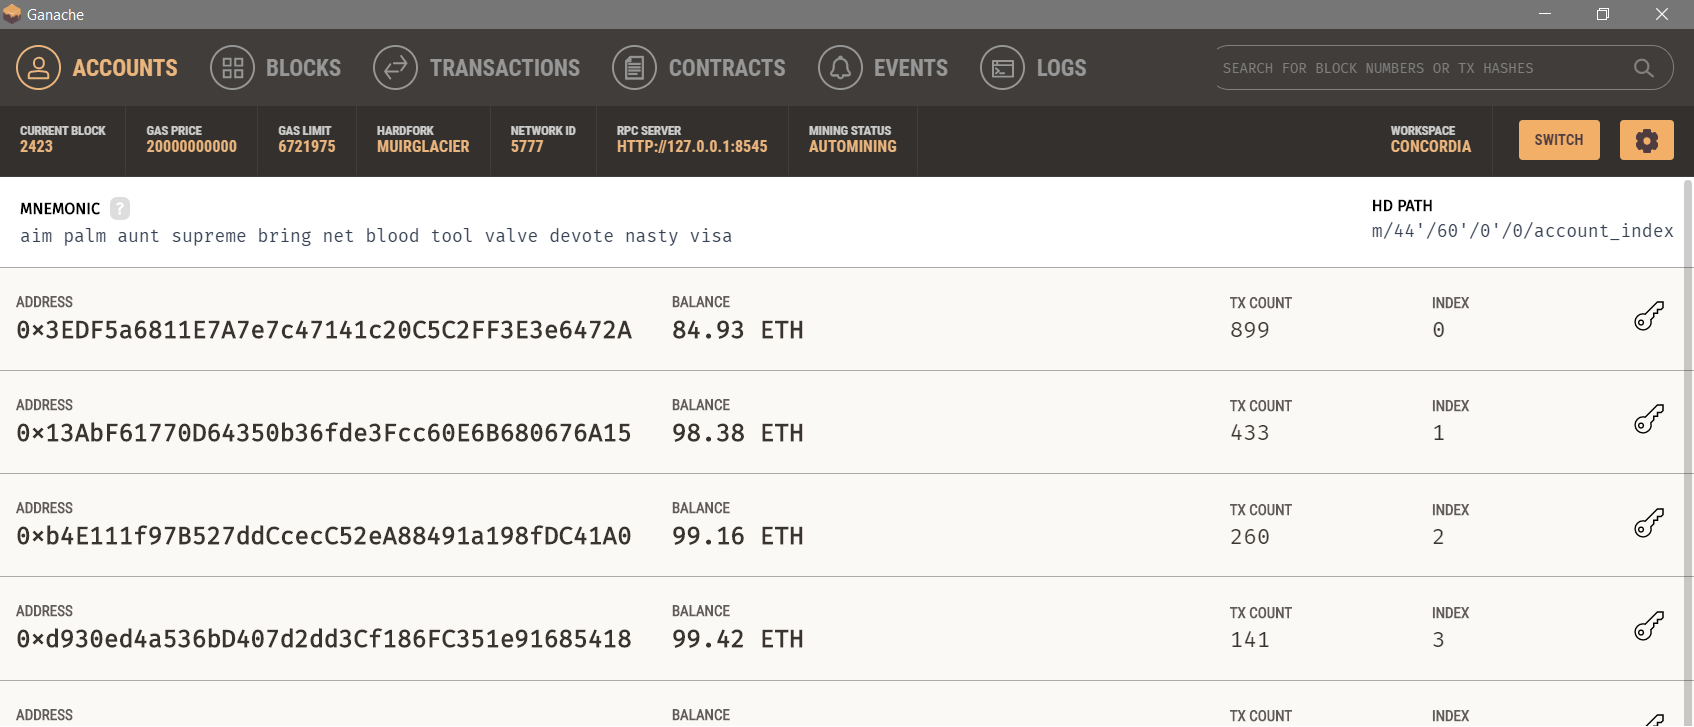
\includegraphics[width=.95\textwidth]{assets/figures/chapter-4/4.2.ganache-gui}
	\caption{Ganache (desktop εφαρμογή)}
\end{figure}

Το Ganache έχει το αποθετήριό του στο GitHub \footnote{\url{https://github.com/trufflesuite/ganache}} και διατίθεται μέσω του μητρώου npm \footnote{\url{https://www.npmjs.com/package/ganache}}.

\subsection{Τεχνολογίες σχετικές με το IPFS}

Σε αυτήν την υποενότητα περιγράφονται όσες τεχνολογίες σχετίζονται με το IPFS (βλ. ενότητα \ref{section:2-7-ipfs}), δηλαδή με το Data tier της τεχνολογικής στοίβας της εφαρμογής.

\subsubsection{js-ipfs} \label{subsection:4-2-4-1-js-ipfs}

\logo{chapter-4/4.2.js-ipfs-logo}{js-ipfs logo}

H υλοποίηση του IPFS που χρησιμοποείται στην εφαρμογή Concordia είναι αυτή σε JavaScript και ονομάζεται js-ipfs. Μέσω αυτής της βιβλιοθήκης, παρέχεται η δυνατότητα δημιουργίας ενός IPFS κόμβου, τόσο σε έναν Node.js server, όσο και σε ένα περιβάλλον browser.

Το js-ipfs έχει το αποθετήριό του στο GitHub\footnote{\url{https://github.com/ipfs/js-ipfs}} και διατίθεται μέσω του μητρώου npm\footnote{\url{https://www.npmjs.com/package/ipfs}}.

\subsubsection{OrbitDB} \label{subsection:4-2-4-2-orbit-db}

\logo{chapter-4/4.2.orbitdb-logo}{OrbitDB logo}

Η OrbitDB είναι μία P2P βάση δεδομένων ανοιχτού κώδικα. Χρησιμοποιεί το IPFS για την αποθήκευση των δεδομένων και το IPFS Pubsub για τον αυτόματο συγχρονισμό των βάσεων δεδομένων μεταξύ των peer. Είναι τελικά συνεπής (eventually consistent) και χρησιμοποιεί CRDTs (Conflict-Free Replicated Data Types) για συγχωνεύσεις βάσεων δεδομένων χωρίς συγκρούσεις, πράγμα που την καθιστά εξαιρετική επιλογή για DApps και offline-first web applications.\cite{4.2-orbitdb}

Κάποια βασικά χαρακτηριστικά της είναι τα εξής:
\begin{itemize}
	\item \textbf{Stores}: Η OrbitDB παρέχει διάφορους τύπους βάσεων (stores) για διαφορετικά μοντέλα δεδομένων και περιπτώσεις χρήσης:
	
	\begin{itemize}
		\item log: ένα αμετάβλητο (μόνο για προσάρτηση) ημερολόγιο με ανιχνεύσιμο ιστορικό.
		\item feed: ένα μεταβλητό αρχείο καταγραφής με ανιχνεύσιμο ιστορικό, του οποίου οι καταχωρήσεις μπορούν να προστεθούν και να αφαιρεθούν.
		\item keyvalue: μία βάση δεδομένων κλειδιών-τιμών.
		\item docs: μία βάση δεδομένων εγγράφων στην οποία μπορούν να αρχειοθετηθούν έγγραφα JSON με ένα καθορισμένο κλειδί.
		\item counter: μία βάση δεδομένων για καταμέτρηση συμβάντων.
	\end{itemize}
	
	Όλα τα store υλοποιούνται πάνω στο \texttt{ipfs-log}, μία αμετάβλητη, operation-based CRDT για κατανεμημένα συστήματα, ενώ υπάρχει και η δυνατότητα δημιουργίας προσαρμοσμένων store ανάλογα με την περίπτωση.
	
	\item \textbf{Address}: Κάθε βάση δεδομένων λαμβάνει κατά τη δημιουργία της μία διεύθυνση της μορφής \texttt{/orbitdb/CID/DATABASE\_NAME}, όπου \texttt{CID} είναι το IPFS multihash του μανιφέστου της και \texttt{DATABASE\_NAME} το όνομα της βάσης.\cite{4.2-orbitdb-guide}Το μανιφέστο είναι ένα IPFS object που περιέχει πληροφορίες της βάσης όπως το όνομα, τον τύπο και έναν δείκτη στον ελεγκτή πρόσβασης (access controller).
	
	\item \textbf{Identity}: Κάθε φορά που προστίθεται μία εγγραφή στη βάση υπογράφεται από τον δημιουργό της, ο οποίος προσδιορίζεται από μία ταυτότητα (identity). Το Identity object, πέρα από τον προεπιλεγμένο τρόπο λειτουργίας, μπορεί να προσαρμοστεί έτσι ώστε να συνδέεται με κάποιο εξωτερικό αναγνωριστικό.
	Η μορφή του έχει ως εξής\footnote{Βλ. και \url{https://github.com/orbitdb/orbit-db-identity-provider}}:
	
	\begin{enumitemcenteredfigure}
		\simplelisting[width=.95\textwidth]{orbit-db-identity.js}
		\caption{OrbitDB Identity}
		\label{figure:4-2-4-2-orbit-db-identity}
	\end{enumitemcenteredfigure}

	\item \textbf{Access Control}: Κατά τη δημιουργία μίας βάσης μπορούν να οριστούν όσοι θα έχουν δικαίωμα εγγραφής σε αυτή, μέσω ενός ελεγκτή πρόσβασης (access controller). Ο ελεγκτής θα περιλαμβάνει τα public key τους, τα οποία μπορούν να ανακτηθούν από το identity του καθενός. Από προεπιλογή και αν δεν ορίζεται διαφορετικά, δίνεται πρόσβαση εγγραφής μόνο στον δημιουργό της βάσης.
\end{itemize}

Η OrbitDB έχει το αποθετήριό της στο GitHub\footnote{\url{https://github.com/orbitdb/orbit-db}} και διατίθεται μέσω του μητρώου npm\footnote{\url{https://www.npmjs.com/package/orbit-db}}.

\subsubsection{Libp2p} \label{subsection:4-2-4-3-libp2p}

\logo{chapter-4/4.2.libp2p-logo}{Libp2p logo}

Η libp2p είναι ένα αρθρωτό σύστημα πρωτοκόλλων, προδιαγραφών και βιβλιοθηκών που επιτρέπουν την ανάπτυξη p2p εφαρμογών. Αποτελεί το υποκείμενο επίπεδο δικτύου του IPFS.\cite{2.7-ipfs-docs}

Ένα από τα υλοποιημένα πρωτόκολλα μεταφοράς δεδομένων της libp2p είναι το libp2p-webrtc-star\footnote{\url{https://github.com/libp2p/js-libp2p-webrtc-star}}. Αποτελεί πρωτόκολλο μεταφοράς δεδομένων το οποίο υποστηρίζεται τόσο από Node.js servers, όσο και από browsers. Περιλαμβάνει, επίσης, έναν signalling server, που επιτρέπει τη γρήγορη ανακάλυψη και διασύνδεση των peers.

Το libp2p-webrtc-star έχει το αποθετήριό του στο GitHub\footnote{\url{https://github.com/libp2p/js-libp2p-webrtc-star}} και διατίθεται μέσω του μητρώου npm\footnote{\url{https://www.npmjs.com/package/libp2p-webrtc-star}}.


